% !TeX program = xelatex 
\documentclass{hitreport}
\usepackage{url}
\usepackage{algorithm,float}  
\usepackage{algpseudocode}  
\usepackage{amsmath}
\usepackage{cite}
\usepackage{threeparttable}
\usepackage{subfig}
\usepackage{listings} %插入代码
\usepackage{xcolor} %代码高亮
\usepackage{tikz}
\usepackage{hyperref}
\usepackage{wasysym}
\usepackage{pgfplots}
\usetikzlibrary{positioning}




\lstset{numbers=left, %设置行号位置
	numberstyle=\tiny, %设置行号大小
	keywordstyle=\color{blue}, %设置关键字颜色
	commentstyle=\color[cmyk]{1,0,1,0}, %设置注释颜色
	frame=single, %设置边框格式
	escapeinside=``, %逃逸字符(1左面的键),用于显示中文
	breaklines, %自动折行
	extendedchars=false, %解决代码跨页时,章节标题,页眉等汉字不显示的问题
	xleftmargin=2em,xrightmargin=2em, aboveskip=1em, %设置边距
	tabsize=4, %设置tab空格数
	showspaces=false %不显示空格
}

\renewcommand{\algorithmicrequire}{\textbf{Input:}}  % Use Input in the format of Algorithm  
\renewcommand{\algorithmicensure}{\textbf{Output:}} % Use Output in the format of Algorithm  

\makeatletter
\newenvironment{breakablealgorithm}
  {% \begin{breakablealgorithm}
   \begin{center}
     \refstepcounter{algorithm}% New algorithm
     \hrule height.8pt depth0pt \kern2pt% \@fs@pre for \@fs@ruled
     \renewcommand{\caption}[2][\relax]{% Make a new \caption
       {\raggedright\textbf{\ALG@name~\thealgorithm} ##2\par}%
       \ifx\relax##1\relax % #1 is \relax
         \addcontentsline{loa}{algorithm}{\protect\numberline{\thealgorithm}##2}%
       \else % #1 is not \relax
         \addcontentsline{loa}{algorithm}{\protect\numberline{\thealgorithm}##1}%
       \fi
       \kern2pt\hrule\kern2pt
     }
  }{% \end{breakablealgorithm}
     \kern2pt\hrule\relax% \@fs@post for \@fs@ruled
   \end{center}
  }
\makeatother

% =============================================
% Part 0 Edit the info
% =============================================

\major{计算机科学与技术}
\name{孙骁}
\title{视听觉信号处理\\实验报告}
\stuid{1180300811} % 学号
\college{计算学部}
\date{2020年12月16日}
\lab{格物207} %实验地点
\course{视听觉信号处理}
\instructor{郑铁然}
% \grades{}
\expname{语音信号端点检测} %实验名称
% \exptype{} % 实验类型
% \partner{} % 同组学生名字
\term{2020秋季学期}

\begin{document}

\maketitle

\tableofcontents
\newpage
% =============================================
% Part 1 Header
% =============================================



% =============================================
% Part 2 Main document
% =============================================

\section{实验目标和内容}

\subsection{实验目标}
\begin{enumerate}
\item 掌握相关语音编辑处理工具软件的操作;
\item 能够编写算法提取语音信号的能量、过零率等特征值;
\item 能够编写算法实现语音信号的端点检测任务。
\end{enumerate}

\subsection{实验内容}
\begin{enumerate}
\item 语音编辑和处理工具的使用
\begin{enumerate}
\item 使用该工具(推荐为CoolEdit pro)打开并显示“1.wav”的波形文件,拷屏贴图到实验报告中;
\item 查看该语音的语谱图,拷屏贴图到实验报告中;
\item 通过听辩,在当前窗口显示该语音信号中第一个音节的时域波形,拷屏贴图到实验报告中;
\item 在实验报告中记录该语音数据的“采样频率”、“量化比特数”和“声道个数”等参数(注:显示在屏幕的右下角)。
\end{enumerate}

\item 能量和过零率特征的提取
\begin{enumerate}
\item 逐一检查各实验语料(共10个wav文件);
\item 编写从wav文件中读入数据的程序。wav文件有44个byte的文件头,可直接跳过,后面就是各采样点,按序排列,每个占用两个byte;
\item 逐帧读入语音数据,帧长设置为256个采样点,无帧叠。根据公式计算每帧的能量和过零率值,将其存储在数组中,并保存在文本文件中。每个语料文件生成一个能量文件和一个过零率文件,文件名为语料文件名加“\_en.txt”和“\_zero.txt”,如对“1.wav”语料生成“1\_en.txt”和“1\_zero.txt”。在文本文件中,每一帧的能量(过零率)值占1行;
\item 提交这些特征文本文件(电子版)作为实验报告的附件。
\end{enumerate}

\item 端点检测算法的实现
\begin{enumerate}
\item 设计端点检测算法,提供如下两种思路,也可以采用其它方法和策略。
\begin{enumerate}
\item 找语音部分,可采用双门限法(见课程PPT);
\item 找静音部分,能量小于某一门限,且连续持续若干帧。
\end{enumerate}
\item 对数据进行仔细分析,调整门限,确定各帧的标签(语音/静音);
\item 根据标签,生成新语料文件,只包含语料的部分。新的语料文件为RAW格式,采用“.pcm”为文件后缀。不包含文件头,直接按序存储各采样点;
\item 提交各新语料文件作为实验报告附件。

\end{enumerate}

\item 计算检测正确率
\begin{enumerate}
\item 打开新生成的语料文件进行听辩,(注:由于是RAW格式,必须正确设置采样频率、量化bit数,声道数等参数);
\item 根据如下信息判断是否检测正确
\begin{enumerate}
\item 是否已经没有残留的静音?
\item 语音内容保留的是否完整?
\end{enumerate}
\item 在实验报告中记录正确的文件数目。
\end{enumerate}


\end{enumerate}

\section{实验环境}

\begin{enumerate}
\item Anaconda 4.8.4
\item Python 3.7.4
\item PyCharm 2020.3 (Professional Edition)
\item Windows 10 2004
\end{enumerate}

\section{实验原理}

\subsection{语音的短时能量}\label{sec:energy}

语音信号的能量随时间变化比较明显,一般清音部分的能量要比浊音部分的能量小得多。对于信号$\left\{x\left(n\right)\right\}$,短时能量的定义为
\begin{align}
\begin{split}
E_n &= \sum_{m=-\infty}^{\infty}\left[x\left(m\right)w\left(n-m\right)\right]^2\\
&=\sum_{m=-\infty}^{\infty}x^2\left(m\right)h\left(n-m\right)\\
&=x^2\left(n\right)\ast h\left(n\right),
\end{split}
\end{align}
其中,$h\left(n\right) = w^2\left(n\right)$,$E_n$表示在信号的第\textit{n}个点开始加窗函数时的短时能量。可以看出,短时能量可以看做是语音信号的平方经过一个线性滤波器的输出,该线性滤波器的单位冲激响应为$h\left(n\right)$,如图(\ref{fig:energy})所示。
\begin{figure}[htb]
\centering
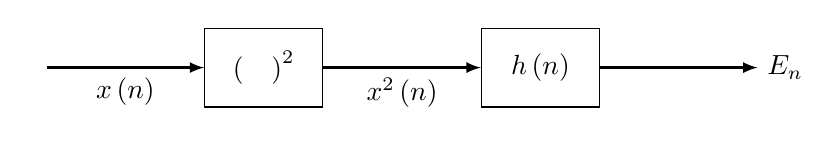
\begin{tikzpicture}[node distance=2cm, auto]
	\node (00) {};
	\node[rectangle, draw, right=of 00 , minimum height=1cm, minimum width=1.5cm] (re1) {$\left(\quad\right)^2$};
	\node[rectangle, draw, right=of re1, minimum height=1cm, minimum width=1.5cm] (re2) {$h\left(n\right)$};			
	\node[right=of re2] (01) {$E_n$};

	\draw[-latex, thick] (00) -- node[below] {$x\left(n\right)$} (re1);
	\draw[-latex, thick] (re1) -- node[below] {$x^2\left(n\right)$} (re2);
	\draw[-latex, thick] (re2) -- (01);
	
\end{tikzpicture}
\caption{短时能量计算的过程}\label{fig:energy}
\end{figure}

冲激响应$h\left(n\right)$的选择决定了短时能量表示方法的特点,理想的结果是存在一个短时窗(冲激响应)以响应快速的幅值变化。如果用$x_w\left(n\right)$表示$x\left(n\right)$经过加窗处理后的信号,窗函数的长度为\textit{N},则短时能量可以表示为
\begin{align}
E_n = \sum_{m=n}^{n+N-1}x_w^2\left(m\right)
\end{align}

\subsection{短时平均过零率}\label{sec:zero}

短时平均过零率是每帧内信号通过零值的次数。对于连续的语音信号,考虑的是时域波形通过时间轴的情况;对于离散信号,考虑的是信号采样点符号变化的次数。通过短时平均过零率可以在一定程度上反应频谱特性。短时平均过零率的公式为
\begin{align}
\begin{split}
Z_n &= \frac{1}{2} \sum_{m=-\infty}^{\infty} \lvert \text{sgn}\left[x\left(m\right)\right] - \text{sgn}\left[x\left(m-1\right)\right] \rvert w\left(n-m\right)\\
&=\frac{1}{2}\sum_{m=n}^{n+N-1} \lvert \text{sgn}\left[x_w\left(m\right)\right] - \text{sgn}\left[x_w\left(m-1\right)\right] \rvert
\end{split}
\end{align}
式中,$\text{sgn}\left[\cdot\right]$是符号函数,即
\begin{align}
\text{sgn}\left[x\left(n\right)\right] = \left\{ \begin{array}{l}
	1,\quad\quad x\left(n\right)\ge 0\\
	-1,\quad\, x\left(n\right)<0\\
\end{array} \right. 
\end{align}

图(\ref{fig:zero})给出了计算短时平均过零率的过程,首先对语音信号序列$x\left(n\right)$进行成对处理,检查是否有过零现象,若符号变化,则表示由一次过零现象;然后进行一阶差分计算,取绝对值;最后进行低通滤波。

\begin{figure}[htb]
\centering
\begin{tikzpicture}[node distance=1cm, auto]
	\node (00) {};
	\node[rectangle, draw, right=of 00 , minimum height=1cm, minimum width=1.5cm] (re1) {成对处理};
	\node[rectangle, draw, right=of re1, minimum height=1cm, minimum width=1.5cm] (re2) {一阶差分};
	\node[rectangle, draw, right=of re2, minimum height=1cm, minimum width=1.5cm] (re3) {$\lvert \quad \rvert$};		
	\node[rectangle, draw, right=of re3, minimum height=1cm, minimum width=1.5cm] (re4) {低通滤波器};	
	\node[right=of re4] (01) {$Z_n$};
	
	\draw[-latex, thick] (00) -- node[below] {$x\left(n\right)$} (re1);
	\draw[-latex, thick] (re1) -- (re2);
	\draw[-latex, thick] (re2) -- (re3);
	\draw[-latex, thick] (re3) -- (re4);
	\draw[-latex, thick] (re4) -- (01);
\end{tikzpicture}
\caption{短时平均过零率计算过程}\label{fig:zero}
\end{figure}


\subsection{端点检测算法}\label{sec:detect}

采用双门限法,利用了章节\ref{sec:energy}的短时能量和章节\ref{sec:zero}的短时平均过零率。\cite{韩纪庆2019}

首先根据浊音情况下的短时平均能量确定阈值参数threshold\_high,根据threshold\_high可以判定语音的前后两点$A_1$和$A_2$,在$A_1$和$A_2$之间的为浊音。再根据较低的阈值参数threshold\_low,由$A_1$点向前找,当短时能量减小到threshold\_low时,可确定点$B_1$;由$A_2$点向后找,同理确定$B_2$点。在$B_1$到$B_2$之间为语音段。然后由$B_1$向前和$B_2$向后,利用短时平均过零率进行搜索。根据无声的情况设置过零率检测阈值threshold\_zero\_cross,又$B_1$向前搜索,如果短时平均过零率大于threshold\_zero\_cross的3倍,则认为信号仍为语音段,直到短时平均过零率下降到低于threshold\_zero\_cross的3倍,此时认为点$C_1$为语音的精确起点。同理可以由$B_2$向后确定语音的终点$C_2$ 。图例如图(\ref{fig:detect})所示。

\begin{figure}
\centering
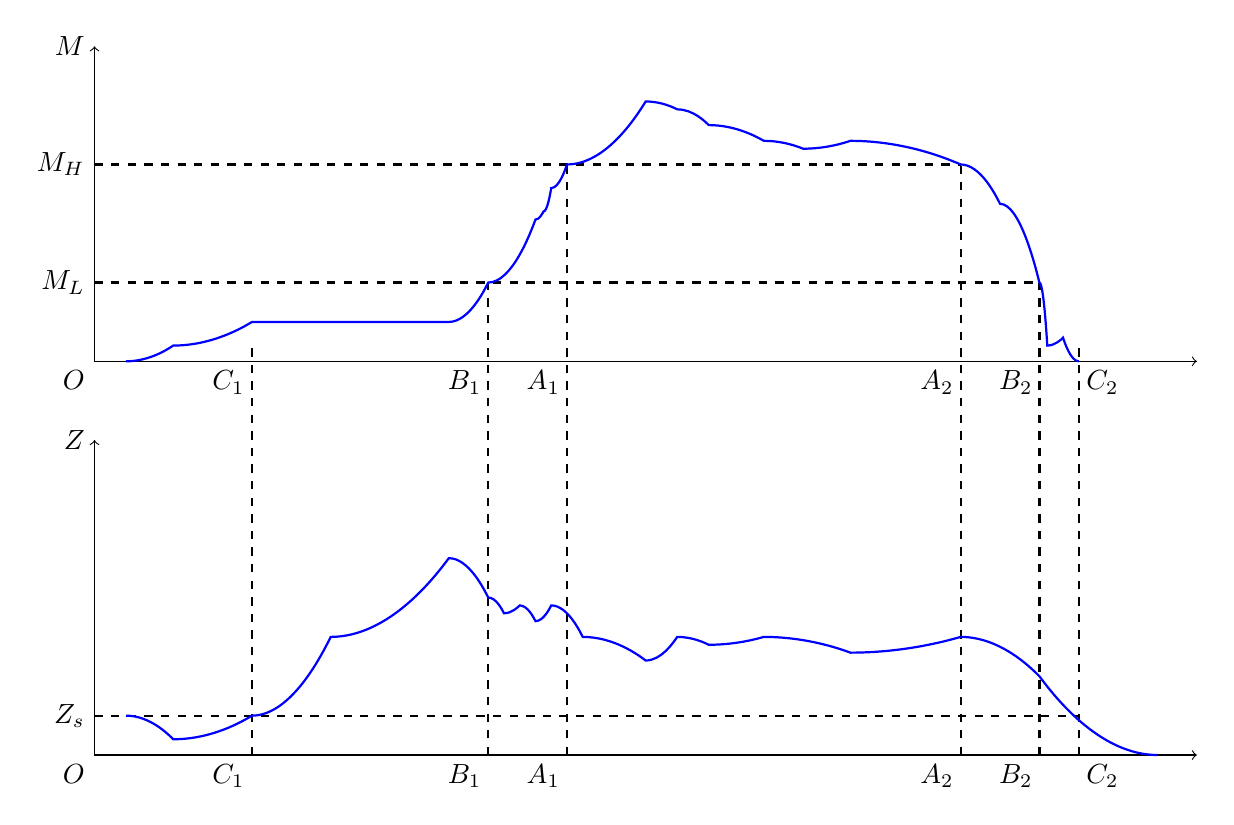
\begin{tikzpicture}
\draw [<->] (0,9) node [left] {$M$} -- (0,5)
node [below left] {$O$} -- (14,5) node [below] {};

\draw [<->] (0,4) node [left] {$Z$} -- (0,0)
node [below left] {$O$} -- (14,0) node [below] {};

\draw (0,0.5) node [left] {$Z_s$};
\draw (0,6) node [left] {$M_L$};
\draw (0,7.5) node [left] {$M_H$};
\draw (1.7,0) node [below] {$C_1$};
\draw (4.7,0) node [below] {$B_1$};
\draw (5.7,0) node [below] {$A_1$};
\draw (10.7,0) node [below] {$A_2$};
\draw (11.7,0) node [below] {$B_2$};
\draw (12.8,0) node [below] {$C_2$};

\draw (1.7,5) node [below] {$C_1$};
\draw (4.7,5) node [below] {$B_1$};
\draw (5.7,5) node [below] {$A_1$};
\draw (10.7,5) node [below] {$A_2$};
\draw (11.7,5) node [below] {$B_2$};
\draw (12.8,5) node [below] {$C_2$};

\draw [black,thick, dashed] (0,0.5) -- (12.5,0.5);
\draw [black,thick, dashed] (0,6) -- (12,6);
\draw [black,thick, dashed] (0,7.5) -- (11,7.5);

\draw [black,thick, dashed] (2,0) -- (2,5.2);
\draw [black,thick, dashed] (5,0) -- (5,6);
\draw [black,thick, dashed] (6,0) -- (6,7.5);
\draw [black,thick, dashed] (11,0) -- (11,7.5);
\draw [black,thick, dashed] (12,0) -- (12,6);
\draw [black,thick, dashed] (12.5,0) -- (12.5,5.2);

\draw [blue,thick] (0.4,0.5) parabola (1,0.2) parabola(2,0.5) parabola (3,1.5) parabola (4.5,2.5) parabola (5,2) parabola (5.2,1.8) parabola (5.4,1.9) parabola (5.6,1.7) parabola (5.8,1.9) parabola (6.2,1.5) parabola (7,1.2) parabola (7.4,1.5) parabola (7.8,1.4) parabola (8.5,1.5) parabola (9.6,1.3) parabola (11,1.5) parabola (12,1) parabola[bend at end] (13.5,0);

\draw [blue,thick] (0.4,5) parabola (1,5.2) parabola(2,5.5) parabola (3,5.5) parabola (4.5,5.5) parabola (5,6) parabola (5.6,6.8) parabola (5.7,6.9) parabola (5.8,7.2) parabola (6,7.5) parabola (7,8.3) parabola (7.4,8.2) parabola (7.8,8) parabola (8.5,7.8) parabola (9,7.7) parabola (9.6,7.8) parabola (11,7.5) parabola (11.5,7) parabola (12,6) parabola (12.1,5.2) parabola (12.3,5.3) parabola[bend at end] (12.5,5);

\end{tikzpicture}
\caption{利用短时能量和短时平均过零率端点检测}\label{fig:detect}
\end{figure}

端点检测算法的代码见附录。

\section{实验步骤及相应结果}

此部分内容与word模板相应章节对应,单击图片引用序号可以跳转查看相应图片结果。

\subsection{语音编辑和处理工具的使用}

\subsubsection{语音文件的时域波形截图}

使用Cool Edit打开 1.wav 文件,结果如图(\ref{fig:1wavtime})所示:

\begin{figure}[htb]
	\centering
	\includegraphics[width=0.9\linewidth]{1_1.png}
	\caption{1.wav的波形文件}\label{fig:1wavtime}
\end{figure}

\subsubsection{语音文件的语谱图截图}

点击功能栏第三组的第一个按钮,Toogle between Spectral and Waveform views,即可得到1.wav的语谱图,如图(\ref{fig:1wavpin})所示。

\begin{figure}[htb]
	\centering
	\includegraphics[width=0.9\linewidth]{1_2.png}
	\caption{1.wav的语谱图}\label{fig:1wavpin}
\end{figure}

\subsubsection{第一个音节的时域波形截图}

在时域波形下选中第一个音节,放大后的结果如图(\ref{fig:firstwav})所示。

\begin{figure}[htb]
	\centering
	\includegraphics[width=0.9\linewidth]{1_3.png}
	\caption{1.wav第一个音节的时域波形}\label{fig:firstwav}
\end{figure}

\subsubsection{语料的格式}\label{sec:infor}

点击功能栏第二组的第十个按钮,Convert Sample Type,可以对音频进行格式转换,最开始显示的即是音频的格式,如图(\ref{fig:wavtype})所示。

\begin{figure}[htb]
	\centering
	\includegraphics[width=0.8\linewidth]{1_4.png}
	\caption{1.wav格式}\label{fig:wavtype}
\end{figure}

由图(\ref{fig:wavtype})可知,音频的采样频率为16000Hz,量化比特数为16位,声道为Mono,即单声道。

\subsection{能量和过零率特征提取}\label{sec:sec2}

\subsubsection{能量特征提取}

实现章节\ref{sec:energy}能量计算方法,在实验中,取帧长为256,即$N=256$,计算能量的核心代码如下:
\begin{lstlisting}[language=python]
def calculate_energy(self):
    energy_dic = {}
    for key in self.wav_data_dic.keys():
        print(f'calculate energy of wav {key}.')
        sample_number = len(self.wav_data_dic[key][4])
        frame_number = math.ceil(sample_number / self.__frame_length)
        energy_of_key = []
        start = 0
        for i in range(frame_number):
            end = min(start + self.__frame_length, sample_number)
            sum_ = reduce(lambda x, y: x + y, (
                map(lambda x: pow(x, 2) * pow(1.0 / self.__frame_length, 2), self.wav_data_dic[key][4][start:end])))
            # print(sum_)
            start += self.__frame_length
            energy_of_key.append(sum_)
        energy_dic[key] = energy_of_key
    return energy_dic
\end{lstlisting}

构造了一个名为energy\_dic的字典,key为10个语料的名称,value为一个列表,名为energy\_of\_key,存储相应语料的能量。

和章节\ref{sec:zero}的过零率计算方法,取帧长为256,即$N=256$,计算短时平均过零率的核心代码如下:
\begin{lstlisting}[language=python]
def calculate_zero_crossing_rate(self):
    zero_rate = {}
    for key in self.wav_data_dic.keys():
        print(f'calculate zero crossing rate of wav {key}.')
        sample_number = len(self.wav_data_dic[key][4])
        frame_number = math.ceil(sample_number / self.__frame_length)
        start = 0
        zero_rate_of_key = []
        for i in range(frame_number):
            sum_ = 0
            end = min(start + self.__frame_length, sample_number)
            for j in range(start, end):
                sum_ += int(self.wav_data_dic[key][4][j]) * int(self.wav_data_dic[key][4][j - 1]) < 0
            start += self.__frame_length
            zero_rate_of_key.append(sum_ / (self.__frame_length - 1))
        zero_rate[key] = zero_rate_of_key
    return zero_rate
\end{lstlisting}

构造了一个名为zero\_rate的字典,key为10个语料的名称,value为一个列表,存储相应语料的短时过零率。


\subsection{端点检测算法}\label{sec:sec3}

端点检测算法采用双门限法,实现章节\ref{sec:detect}的算法,代码见附录,生成的检测文件见附件。

\subsection{计算检测正确率}\label{sec:sec4}

\subsubsection{“1.wav”语料去除静音后的时域波形截图}

去除静音后的1.wav时域波形如图(\ref{fig:41})所示。

\begin{figure}[htb]
	\centering
	\includegraphics[width=0.9\linewidth]{4_1.png}
	\caption{1.wav第一个音节的时域波形}\label{fig:41}
\end{figure}

\subsubsection{正确率}

首先将端点检测后的语料的时域波形与原语料的时域波形进行比较,结果如图(\ref{fig:test1})和图(\ref{fig:test2})所示。对生成的pcm文件进行打开,按照章节\ref{sec:infor}的信息对生成的语料进行格式选择,经过听音辨认,检测准确率达到100\%。

\begin{figure}[htb]
	\centering
	\subfloat[语料1时域波形]{
		\label{fig:1}\includegraphics[width=.4\textwidth]{1_1.png}}\hspace{20pt}
	\subfloat[端点检测后语料1时域波形]{
		\label{fig:1re}\includegraphics[width=.4\textwidth]{4_1.png}}
	\\
	\subfloat[语料2时域波形]{
		\label{fig:2}\includegraphics[width=.4\textwidth]{2_2.png}}\hspace{20pt}
	\subfloat[端点检测后语料2时域波形]{
		\label{fig:2re}\includegraphics[width=.4\textwidth]{4_2.png}}
	\\
	\subfloat[语料3时域波形]{
		\label{fig:3}\includegraphics[width=.4\textwidth]{2_3.png}}\hspace{20pt}
	\subfloat[端点检测后语料3时域波形]{
		\label{fig:3re}\includegraphics[width=.4\textwidth]{4_3.png}}
	\\
	\subfloat[语料4时域波形]{
		\label{fig:4}\includegraphics[width=.4\textwidth]{2_4.png}}\hspace{20pt}
	\subfloat[端点检测后语料4时域波形]{
		\label{fig:4re}\includegraphics[width=.4\textwidth]{4_4.png}}
	\\
	\subfloat[语料5时域波形]{
		\label{fig:5}\includegraphics[width=.4\textwidth]{2_5.png}}\hspace{20pt}
	\subfloat[端点检测后语料5时域波形]{
		\label{fig:5re}\includegraphics[width=.4\textwidth]{4_5.png}}
	\caption{语料1\textasciitilde5的时域波形与端点检测后时域波形的对比}\label{fig:test1}
\end{figure}

\begin{figure}[htb]
\centering
	\subfloat[语料6时域波形]{
		\label{fig:6}\includegraphics[width=.4\textwidth]{2_6.png}}\hspace{20pt}
	\subfloat[端点检测后语料6时域波形]{
		\label{fig:6re}\includegraphics[width=.4\textwidth]{4_6.png}}
	\\
	\subfloat[语料7时域波形]{
		\label{fig:7}\includegraphics[width=.4\textwidth]{2_7.png}}\hspace{20pt}
	\subfloat[端点检测后语料7时域波形]{
		\label{fig:7re}\includegraphics[width=.4\textwidth]{4_7.png}}
	\\
	\subfloat[语料8时域波形]{
		\label{fig:8}\includegraphics[width=.4\textwidth]{2_8.png}}\hspace{20pt}
	\subfloat[端点检测后语料8时域波形]{
		\label{fig:8re}\includegraphics[width=.4\textwidth]{4_8.png}}
	\\
	\subfloat[语料9时域波形]{
		\label{fig:9}\includegraphics[width=.4\textwidth]{2_9.png}}\hspace{20pt}
	\subfloat[端点检测后语料9时域波形]{
		\label{fig:9re}\includegraphics[width=.4\textwidth]{4_9.png}}
	\\
	\subfloat[语料10时域波形]{
		\label{fig:10}\includegraphics[width=.4\textwidth]{2_10.png}}\hspace{20pt}
	\subfloat[端点检测后语料10时域波形]{
		\label{fig:10re}\includegraphics[width=.4\textwidth]{4_10.png}}
	\caption{语料6\textasciitilde10的时域波形与端点检测后时域波形的对比}\label{fig:test2}
\end{figure}




\section{实验结论}

\begin{enumerate}
\item 使用双门限法对语音进行端点检测可以较好地区分语音和非语音;
\item 双门限法做语音端点检测时,高低阈值和平均过零率阈值的选取会显著影响最后检测的结果;
\item 使用lambda匿名函数可以有效简化代码。
\end{enumerate}

\renewcommand\refname{参考文献}
 
\renewcommand\refname{参考文献}
 
\bibliographystyle{unsrt} %%参考文献的格式(可选的格式还有:plain)
 
\bibliography{Refer.bib}    %%参考文件存储位置

\newpage
\begin{appendices}

\section{从wav文件读取数据——read\_wav\_from\_file.py}

\lstinputlisting[language=python]{code/read_wav_from_file.py}

\section{对语料计算短时能量值与过零率——energy\_zero\_crossing\_rate\_extract.py}

\lstinputlisting[language=python]{code/read_wav_from_file.py}

\section{对语料端点检测——voice\_endpoint\_detection.py}

\lstinputlisting[language=python]{code/voice_endpoint_detection.py}

\section{将语音短时能量、过零率、端点检测结果写入文件——write\_to\_file.py}

\lstinputlisting[language=python]{code/write_to_file.py}

\end{appendices}

\end{document}
